\section{Product perspective}
\label{sec:product_perspective}%



\subsection{Scenarios}
\label{subsec:scenarios}%
\begin{itemize}
    \item \textbf{Scenario 1 : Companies Submit Internship Postings}

Companies create and publish detailed internship descriptions, specifying roles, qualifications, benefits, and deadlines. They ensure that the postings are tailored to attract the right candidates. Companies can also update these postings to reflect changes or clarify details as needed, ensuring that they remain appealing and informative.
    \item \textbf{Scenario 2 : Students Create Profiles and Upload CVs}

Students register on the platform and complete their profiles by entering academic background, skills, extracurricular activities, and personal preferences for internships. They upload polished and revised CVs that highlight their qualifications, ensuring visibility to potential employers. The platform may also provide guidance on enhancing CV quality to improve students' chances of selection. 
    \item \textbf{Scenario 3 : Students Browse and Apply for Internships} 

Students actively explore the internship database on the platform using filters such as preferred location, required skills, and duration. The system allows students to compare internships and apply to multiple opportunities at the same time, making the application process efficient and maximizing their chances of success.
    \item \textbf{Scenario 4 : \textbf{System Recommends Internships to Students} }

Using advanced matching algorithms, the platform suggests internships that align with the profile, academic qualifications and career goals of the student. These recommendations adapt over time based on student interactions, applications and feedback, creating a highly personalized experience.
\item \textbf{Scenario 5 : \textbf{Companies Receive and Review Applications} }

Companies access a dashboard dedicated to them in order to view applications submitted by students. They evaluate candidates by comparing their profiles and CVs with internship requirements. The platform provides tools to rank applicants, add notes, and collaboratively review candidates with team members.
\item \textbf{Scenario 6 :\textbf{Interview Scheduling and Management}}

The platform simplifies interview logistics by giving companies the opportunity to schedule interviews with selected candidates. Supporting virtual meeting integrations and sending automated reminders to ensure all parties are prepared. The system also tracks the results of the interviews for later reference.
\item \textbf{Scenario 7 : Feedback Collection:} 

Both students and companies submit structured feedback after each major milestone, such as application reviews or interviews. This feedback is used to refine the profiles of students, improve internship postings, and enhance the platform’s recommendation capabilities. Feedback mechanisms also promote transparency and accountability.
\item \textbf{Scenario 8 : \textbf{Internship Monitoring by Universities} }

Universities oversee active internships by receiving updates on student performance, company satisfaction, and project progress. They use dashboards to track multiple internships simultaneously and ensure compliance with educational objectives. Universities can also intervene when problems are reported.
\item \textbf{Scenario 9 : \textbf{Complaint Handling}}

An efficiently working complaint management system allows students and companies to raise concerns during internships. Complaints are directed to universities that investigate and mediate to resolve conflicts. The system records the entire process to ensure fairness and transparency.
\item \textbf{Scenario 10 : \textbf{System Updates Recommendations} }

The platform’s recommendation engine evolves based on user feedback, application trends, and internship results. This dynamic update feature ensures future recommendations are more accurate and relevant, helping both students and companies.
\item \textbf{Scenario 11 : \textbf{Post-Internship Evaluation} }

After completing internships, students and companies provide detailed evaluations of their experiences. These evaluations highlight strengths, areas for improvement, and contribute to building a database of internship performance indicators for future users.
\item \textbf{Scenario 12 : Statistical Data Analysis} 

The platform collects data on applications, student performance, and company satisfaction. Advanced statistical tools analyze these data to uncover trends such as popular skills, successful industries, or common challenges. Insights from these analyses inform strategic improvements.
\item \textbf{Scenario 13 : Notifications and Alerts} 

The platform ensures that users are continuously informed through real-time notifications. Students receive alerts about new internships that match their profiles, upcoming deadlines, or interview schedules. Companies are notified of new applications, interview confirmations, and feedback submissions, ensuring timely responses and actions.
\end{itemize}
\subsection{Class Diagrams}
\label{subsec:class_diagrams}%
\begin{figure}[H]
    \centering
    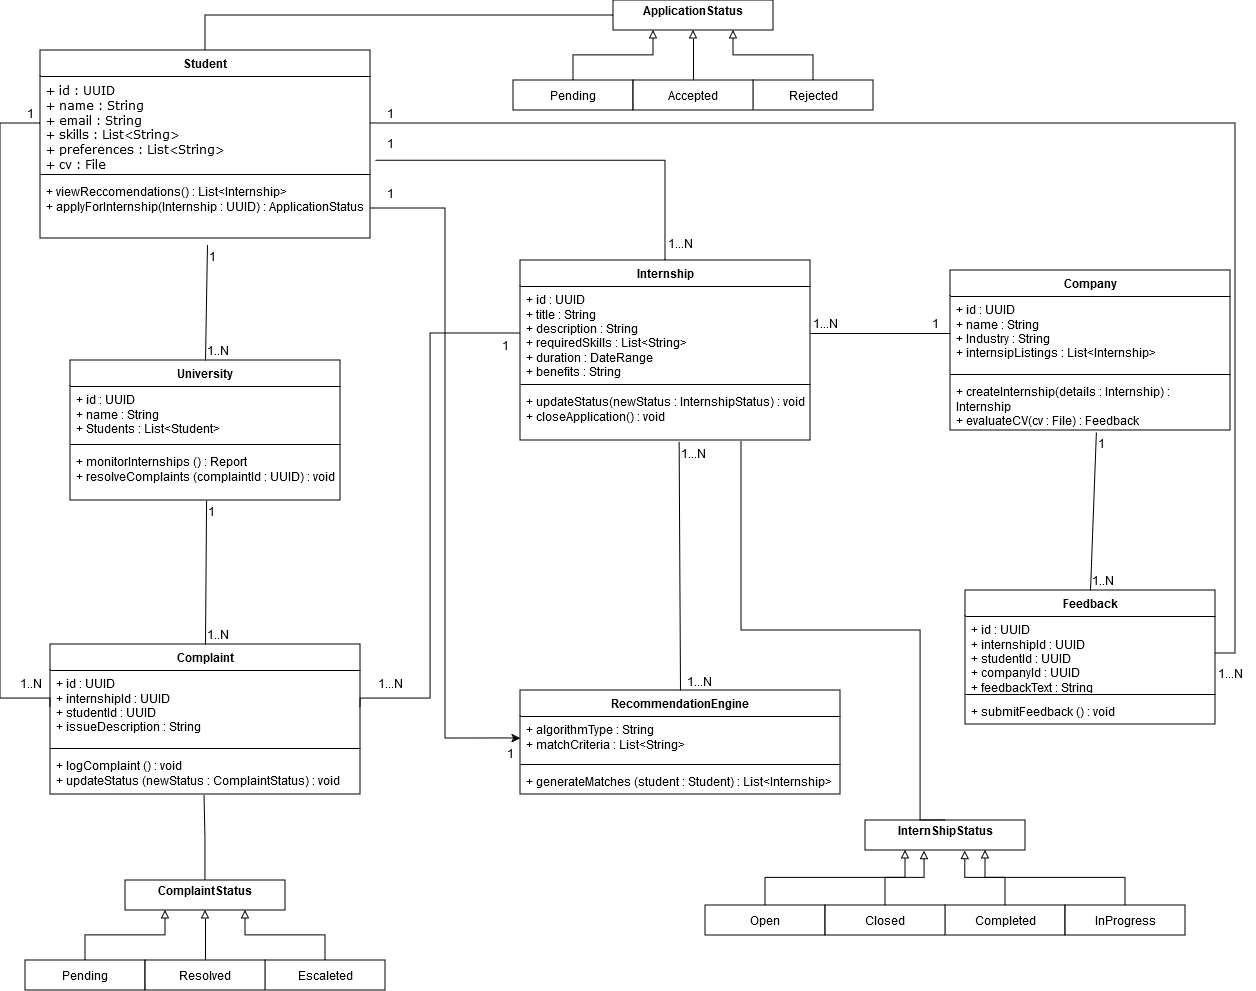
\includegraphics[width=1\linewidth]{Images/Class diagrams/ClassDiagram.png}
    \caption{Class Diagram}
    \label{fig:enter-label}
    
    
\end{figure}

\subsection{State Diagrams}
\label{subsec:class_diagrams}%

\paragraph{Sign-up} Initially, users can create a generic account that allows them to browse available posts without the ability to post. To upgrade to a full account, they must verify their email address, select a role (either as a student or a company), and complete the required fields for their chosen role.

\begin{figure}[H]
    \centering
    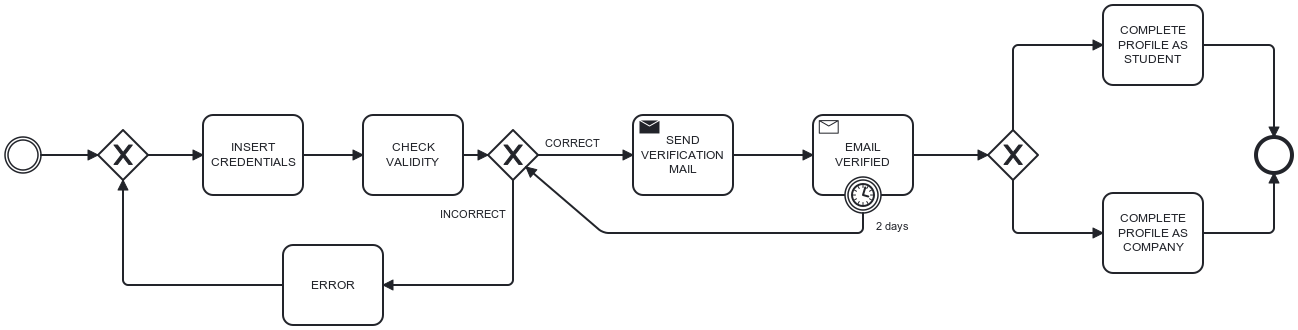
\includegraphics[width=1\linewidth]{Images//state diagrams/SIGNUP.png}
    \caption{Sign-up state diagram}
    \label{fig:enter-label}
\end{figure}

\paragraph{Login} During login, the system verifies the user's credentials to ensure they are correct. Upon successful authentication, the user is redirected to their personalized homepage.

\begin{figure}[H]
    \centering
    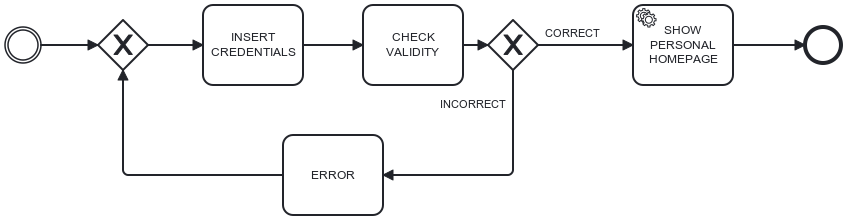
\includegraphics[width=1\linewidth]{Images//state diagrams/LOGIN.png}
    \caption{Login state diagram}
    \label{fig:enter-label}
\end{figure}

\paragraph{Apply for an internship} The student reviews their recommended internships. If they decide to apply for one, they must contact the company, which will proceed to schedule an interview. If the interview is successful and both parties agree, the internship will be communicated to the university.

\begin{figure}[H]
    \centering
    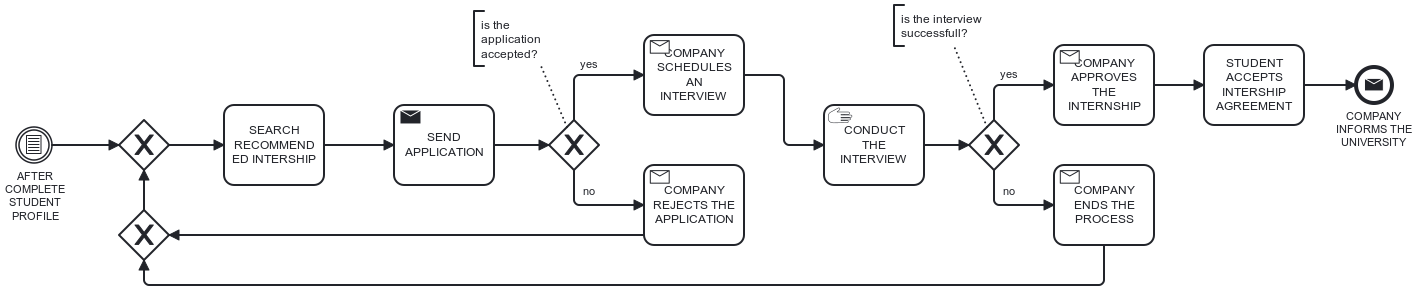
\includegraphics[width=1\linewidth]{Images//state diagrams/APPLICATION.png}
    \caption{Application state diagram}
    \label{fig:enter-label}
\end{figure}

\paragraph{Complaints handling} Both students and companies can submit a complaint during the internship. The university evaluates the complaint to determine whether intervention is necessary. If no intervention is required, the process ends without further action. However, if intervention is necessary, the university attempts to mediate between the parties to resolve the issue. If mediation is successful, the process concludes, and the internship continues as usual. On the other hand, if mediation fails or the issue remains unresolved, the university decides to terminate the internship. Before finalizing the termination, the university ensures that both parties are informed about the decision.

\begin{figure}[H]
    \centering
    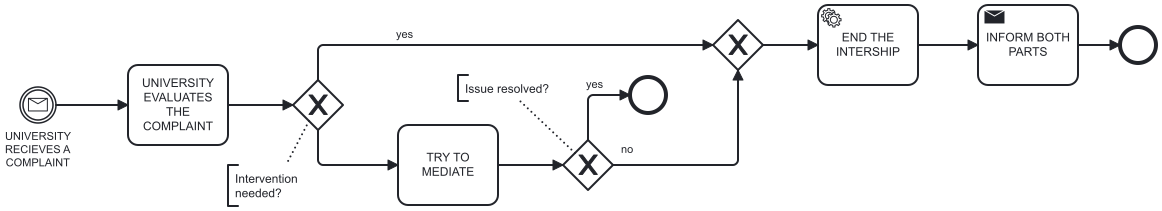
\includegraphics[width=1\linewidth]{Images//state diagrams/COMPLAINTS.png}
    \caption{Complaint diagram}
    \label{fig:enter-label}
\end{figure}

\section{Product functions}
\label{sec:product_functions}%

Here's the main functions of S\&C system:

\paragraph{Register to the platform}
The S\&C platform allows students and companies to register. During the registration process, users are required to provide the following information:
\begin{center}
\renewcommand{\arraystretch}{1}
\begin{tabular}{|p{5cm}|p{5cm}|p{5cm}|}
\hline
\textbf{Field} & \textbf{Required for} & \textbf{Notes} \\
\hline
Role & Both & Student or Company \\
\hline
Full name & Both &  \\
\hline
Company name & Company only &  \\
\hline
Email address & Both & Checking valid email address \\
\hline
Password & Both & Checking security standards \\
\hline
Attending university & Student only & Checking an existing university name \\
\hline
Phone number & Both &  \\
\hline
Postal Code & Both & Matching parameter \\
\hline
Office address & Company only & Matching parameter \\
\hline
Office phone number & Company only & Optional \\
\hline
\end{tabular}
\end{center}

While registering to the system, users must first declare that they have read and understood the Privacy Statement. They are also required to accept the Terms and Conditions, which request consent for the acquisition and processing of their personal data for the purpose of using the platform's matching analysis.

\paragraph{Post an internship}A button within the company's dashboard that opens a form for creating and submitting a new internship posting, including fields for job title, description, requirements, salary, and duration

\paragraph{Check recommended internships}A searchable and filterable page accessible to all users, displaying a list of internships with brief descriptions and company details.
\paragraph{Apply for an internship}A button on each internship's detail page that triggers a form submission, allowing students to send their application with a personalized message and resume upload.
\paragraph{Evaluate an application}A company dashboard feature showing a list of received applications with applicant details, resumes, and the option to accept, reject, or schedule interviews.
\paragraph{Schedule an interview}An action available on an application detail page that opens a scheduling form, allowing the company to set the interview's date, time, and mode.
\paragraph{Submit a complaint}A button in the dashboard (available to students and companies) that opens a form for submitting a formal complaint, including issue details.
\paragraph{Submit a feedback}A post-internship form accessible to both students and companies where they can rate the experience, provide comments, and suggest improvements for future internships.

\section{User characteristics}
\label{sec:user_characteristics}%

The actors of the application are the following:

\begin{itemize}
    \item \textbf{Student}: A single person registered as a student on the platform. Their aim is to find internships aligned with their academic background, skills, and career goals. They need only an active account, an internet connection, and access to a digital CV.
    \item \textbf{Company}: An organization of people registered on the platform. Its goal is to publish internship opportunities, examine applications, and hire suitable candidates. It requires an active account, an internet connection, and major internship details.
    \item \textbf{University}: A career services representative with a passive role on the platform. Universities are contacted only if an internship goes wrong or complaints emerge from companies or students. Their task is to review the situation and, if necessary, interrupt the internship. They need access to relevant student and company data.
\end{itemize}

\section{Assumptions, dependencies and constraints}
\label{sec:assumptions_dependencies_and_constraints}%
\newcounter{da} 
\setcounter{da}{1}
\newcommand{\cda}{D\arabic{da}\stepcounter{da}} 
\begin{center}
    \renewcommand{\arraystretch}{2}
    \begin{longtable}{ l p{0.8\linewidth} } 
        \hline
        \textbf{ID} & \textbf{Description} \\ 
        \hline
        \cda & Internship descriptions are comprehensive and reliable \\ \hline
        \cda & CVs accurately reflect students' skills and experiences \\ \hline
        \cda & Universities actively oversee internships and intervene when necessary \\ \hline
        \cda & Companies manage interview timelines and conduct them professionally \\ \hline
        \cda & Users provide meaningful feedback to improve the system \\ \hline
        \cda & Problems are reported in a timely manner by all parties \\ \hline
        \cda & The platform supports high user traffic without performance issues \\ \hline
        \caption{Domain Assumptions.}
        \label{tab:worldph_tab}%
    \end{longtable}
\end{center}

